\documentclass[fontsize = 12pt, paper = a4]{scrreprt} 

\setlength{\parindent}{0pt}
\usepackage[english,ngerman]{babel}
\usepackage[utf8]{inputenc} 
\usepackage{enumerate}
\usepackage{amssymb,amsmath}

%------------ Überschriften verkleinern und hochsetzen ----------%

%\makeatlettern
%\renewcommand*\@makechapterhead[1]{%
%{\parindent \z@ \raggedright \normalfont
%\LARGE\bfseries
%\ifnum \c@secnumdepth >\m@ne
%\thechapter\space
%\fi
%#1\par\nobreak
%\vskip 20\p@
%}} 

% ------------------------ Blattlayout- -------------------------%

\usepackage {geometry}   
\geometry   {left     = 2.5cm,
             right    = 2.5cm, 
             top      = 1.5cm,
             bottom   = 1.5cm,
             includehead, includefoot}
             
% ------------------------ Seitenstil ---------------------------%           

% Umdefinieren von Befehlen zur Vermeidung von Bugs:

\renewcommand*{\chapterpagestyle}{scrheadings} 
\renewcommand*{\chapterheadstartvskip}{\vspace*{-\topskip}}

% Gestaltung der Kopf- und Fußzeile:

\pagenumbering{arabic}
            
\usepackage[automark]{scrpage2}
\automark[chapter]{section}
\pagestyle{scrheadings} 
\ohead[\pagemark]{\pagemark}
\setlength{\footskip}{5mm} 

\clearscrheadfoot
\lohead{Benutzerhandbuch}
\rohead{\headmark}
\lofoot{Softwareprojekt TU Ilmenau SS 2013}
\rofoot{\pagemark}

% Kopf- und Fußzeilenlinie:

\setheadsepline{.6pt} % Linie für Kopfzeile
\setfootsepline{.6pt} % Linie für Fußzeile 

% Für Unterstreichungen:

\usepackage[normalem]{ulem}

% Buchstabenglättung am Rand:
  
\usepackage {microtype} 

% Bildunterschriften zentrieren:

%\usepackage{caption}
%\captionsetup{margin=10pt,font=small,labelfont=bf, justification = centering}

%-------------------------------------------------------------------%

% Für die Einbindung von Bildern:

\usepackage[pdftex]{graphicx} % .pdf, .png oder .jpg möglich!
\usepackage{rotating}         % Grafiken rotieren

% Nutzung in drei Umgebungen möglich:

% (1) \begin{turn}{Winkel} ...  \end{turn}
% (2) \begin{sideways} ... \end{sideways} 90° im math. pos. Sinn
% (3) \begin{rotate}{Winkel} ... \end{rotate} 
%     ---> 90° im math. pos. Sinn, allerdings keine Platzreservierung 

\usepackage{wrapfig}
%\usepackage{picins}   % Textumflossene Grafiken
\usepackage{subfigure}
\usepackage{floatflt}
\usepackage[justification=centering]{caption}

%-------------------------------------------------------------------%
 
% Packete für Tabellen:

\usepackage{booktabs}
\usepackage{array}    % optional
\usepackage{tabularx} % optional

\usepackage[font=footnotesize,labelfont=bf,singlelinecheck=false,
            format=plain,,justification=justified,indention=0cm]                     {caption} 

\usepackage{setspace}

\usepackage{enumitem} 

%----------------  Anfang des Dokuments ------------------%

\begin{document}

%*******************************************************************%

% Entwurf Titelseite:

\titlehead{\begin{center}
\textbf{\Huge Benutzerhandbuch}
\end{center}}
		   
\title{Service-Interface \\ für ein Formula-Student-Fahrzeug}

\subtitle{Technische Universität Ilmenau \\
		  Softwareprojekt SS 2013 \\ Gruppe 19}			
		
\author{Christian Boxdörfer \\ Thomas Golda \\ Daniel Häger \\ 
		David Kudlek \\  Tom Porzig \\ Tino Tausch \\ 
		Tobias Zehner \\ Sebastian Zehnter}
		
\date{Hier Datum einfügen}	 
	  
\publishers{betreut durch \\ \vspace{1cm} Dr. Heinz-Dietrich Wuttke, TU Ilmenau \\ Oliver Dittrich, fachlicher Betreuer Team StarCraft e.V.}

\maketitle		

%*******************************************************************%

% --------------------- Inhaltsverzeichnis -----------------------%

\begin{spacing}{0.86} 
\tableofcontents
%\setcounter{secnumdepth}{4} % Tiefere Gliederungsebene  
\setcounter{tocdepth}{4} % Anzeige bis Gliederungsstufe 4
%\addtocontents{toc}{\protect\enlargethispage{2\baselineskip}} 
\end{spacing}


\newpage % Seitenumbruch

%--------------------------  Einleitung  ---------------------------%

\chapter{Einleitung}

%----- Installation und Konfiguration des Service Interfaces -------%

\chapter{Installation und Konfiguration des Service Interfaces}


%-------------------------------------------------------------------%
%-------------------------------------------------------------------%

\section{MicroAutoBox II}

Für eine erfolgreiche Installation und Konfiguration der MicroAutoBox II müssen zu Beginn der Installation neben dieser Hardwarekomponente folgende Dateien in MATLAB und Modelle in Simulink vorliegen:

\begin{itemize}

\item \textit{udp\_final.mdl}: Diese Datei beinhaltet das von uns bereitgestellte Simulink-Modell für das Service Interface.

\item \textit{config\_datenpaket.m} Dieses *.m - File enthält die zur Konfiguration des Datenpaketes notwendigen Vektoren, welche je nach Art des Datenpaketes an dieses angepasst werden können und Informationen über dessen Attribute und Zusammensetzung beinhalten (Verweis ED).

\item \textit{signalgenerator\_microautobox.m} Dieses optionale *.m - File dient dazu, den Signalgenerator im Simulink-Modell zu Simulationszwecken mit generierten Testdaten auszustatten, um bei Veränderungen des Simulink-Modells oder bei einer Modifizierung der   auf dem Embedded-PC oder dem virtuellen Server implementierten *.cpp - Dateien eine Verifizierung des Service Interfaces anhand dieser bekannten Testdaten durchführen zu können (Verweis ED).

\end{itemize} 

Falls diese Dateien alle zur Verfügung stehen sollten, ist in einem ersten Schritt das Simulink-Modell \textit{udp\_final.mdl} durch das Programm MATLAB zu öffnen, wonach sich in Simulink auf der obersten Modellebene  folgende Subsysteme befinden (s. Abb. \ref{topmodell}):

\begin{figure}[h]
\centering
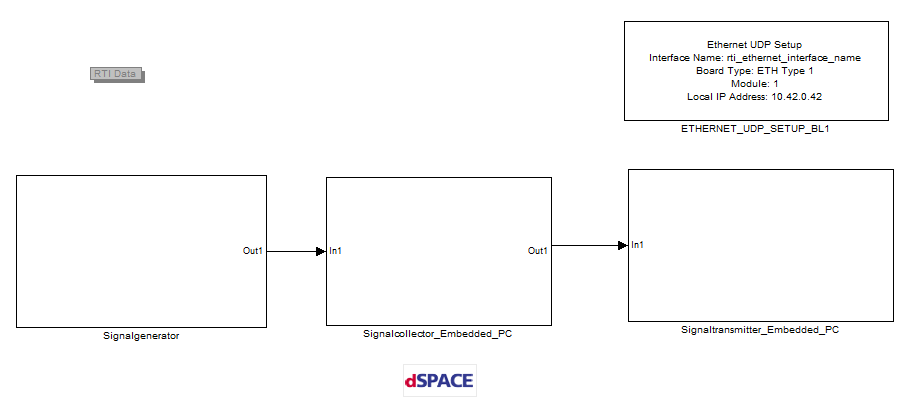
\includegraphics[scale = 0.65]{topmodell}
\caption[Gesamtaufbau Simulink-Modell]{Gesamtaufbau des Simulink-Modells auf höchster Modellebene}
\label{topmodell}
\end{figure} 

\newpage

%-------------------------------------------------------------------%

\subsection{Konfiguration der Ethernet-Schnittstelle}

Daraufhin ist bei der weiteren Vorgehensweise anschließend die Konfiguration der Ethernet-Schnittstelle vorzunehmen. Hierzu öffnet man durch einen Doppelklick den in Abb. \ref{topmodell} zu sehenden Block \textit{"`Ethernet UDP Setup"} ein Fenster, in welchem nun die Möglichkeit besteht, zwischen den beiden Reitern \textit{"`Unit"} und \textit{"`Options"} zu navigieren (Verweis dSPACE Doku) und dort bei den jeweiligen Einstellungen Modifikationen vorzunehmen. Im Folgenden werden obligatorische Änderungen durch ein (*) am jeweiligen Parameter gekennzeichnet. \\

\textbf{Reiter "`Unit"} 

\begin{itemize}

\item \textit{Interface Name}: Hier kann ein selbst gewählter Name für die Schnittstelle festgelegt werden.

\item \textit{$Board \ Type \ ^{(*)}$}: Bei Verwendung der MicroAutoBox II ist dort die Option \\ "`ETH Type 1"\ auszuwählen.

\item \textit{Module number}: Der dortige Wert ist auf "`1" vorkonfiguriert und kann auch so belassen werden.

\item \textit{$Local \ IP \ adress \ ^{(*)}$}: Hier ist die lokale IP-Adresse der MicroAutoBox II in Abhängigkeit des gewählten Subnetzes  anzugeben (z.B. 192.X oder 10.X).

\end{itemize}

\textbf{Reiter "`Options"} \\

In diesem Reiter können anhand nachfolgender Einstellungen bis zu vier verschiedene Sockets innerhalb des Modells definiert werden. Der Socket 1 ist hierbei für das Datenpaket mit den Fahrzeugdaten und der Socket 2 für das Datenpaket mit den Paketinformationen vorgesehen. Darüber hinaus stehen bei beabsichtigten Erweiterungen des Modells Socket 3 und 4 zur freien Verfügung.

\begin{itemize}

\item \textit{$Enable \ ^{(*)}$}: Ein gesetztes Häkchen entscheidet bei diesem Parameter darüber, ob der jeweilige Socket aktiviert oder deaktiviert wird. Es ist notwendig, die Sockets 1 und 2 zu aktivieren, um den Transport der Datenpakete an den Embedded-PC zu ermöglichen (s. o.). Darüber hinaus sollten die Sockets 3 und 4, falls diese nicht anderweitig verwendet werden, deaktiviert werden.  

\item \textit{$Local \ Port \ Number \ [0 \ ... \ 65535] \ ^{(*)}$}: In diesem Feld ist die Nummer des lokalen Ports der MicroAutoBox II einzutragen. 

\item \textit{$Remote \ Port \ Number \ [0 \ ... \ 65535] \ ^{(*)}$}:
Dort muss die Nummer des externen Ports -- also der gewünschte Port des Embedded-PCs -- eingetragen werden. \\ 

\textbf{Anmerkung:} Um Verwechslungen beim Eintragen der Portnummern o.ä. zu vermeiden, ist es empfehlenswert, für beide Ports die selbe Nummer zu vergeben. 

\end{itemize} 

\newpage

Nachdem alle obligatorischen Änderungen vorgenommen wurden, muss in einem nächsten Schritt innerhalb der Subsysteme \textit{UDP\_DATEN} und \textit{UDP\_PAKETINFORMATIONEN} die Blöcke "`ETHERNET\_UDP\_TX\_BL1"\ und "`ETHERNET\_UDP\_TX\_BL2"\ angepasst werden. Um zu diesen Blöcken zu gelangen, verfolgt man in bekannter Weise durch Doppelklicks auf der obersten Modellebene die folgenden Pfade im Modell: 

\begin{itemize}[leftmargin=*]

\item "`ETHERNET\_UDP\_TX\_BL1"\ : \\ Signaltransmitter\_Embedded\_PC $\rightarrow$ UDP\_DATEN 

\item "`ETHERNET\_UDP\_TX\_BL2"\ : \\ Signaltransmitter\_Embedded\_PC $\rightarrow$ UDP\_PAKETINFORMATIONEN

\end{itemize}

Nach dem Öffnen der Einstellungen der beiden Blöcke muss bei dem Parameter "`Maximum Message Size"\ der gleiche Wert eingetragen werden, der auch am Port "`Message Size"\ am jeweiligen Block anliegt. Sollten diese Werte nicht bekannt sein, so können diese an den beiden Displays "`DISPLAY\_MSGSIZE\_DATEN"\ und "`DISPLAY\_MSGSIZE\_PAKETINFO"\ abgelesen werden. Falls dies nach dem Starten der Simulation aufgrund von Fehlermeldungen nicht der Fall sein sollte, müssen die beiden Subsysteme UDP\_DATEN und UDP\_PAKETINFORMATIONEN kurzzeitig vom restlichen Modell abgetrennt / entfernt werden und die ehemals hinführenden Leitungen durch Terminatoren abgeschlossen werden. Anschließend kann der Wert bei Simulationsbeginn abgelesen, die neu eingefügten Terminatoren nach Beenden der Simulation wieder entfernt und die beiden Subsysteme erneut an das restliche Modell an den vorherigen Stellen angeschlossen werden. \\ 

Falls jedoch die genaue Anzahl / die Signalbreite an Fahrzeugdaten bzw. an Paketinformationen bekannt sein sollte, kann die Größe der "`Maximum Message Size"\ auf elegantere Weise ermittelt werden. Da die Werte der Fahrzeugdaten den Datentyp \textit{int16} aufweisen und die Paketdaten den Datentyp \textit{uint8} besitzen, müssen die jeweiligen Signalbreiten nur mit 2 bzw. 1 (Byte) multipliziert werden, um den gesuchten Wert korrekt zu ermitteln \\ (s. die Subsysteme MSGSIZE\_DATEN und MSGSIZE\_PAKETINFO). \\  

\textbf{Anmerkung}: Für weiterführende Informationen und Hinweise empfiehlt es sich, die Dokumentation der Firma dSPACE bzgl. des RTI Ethernet (UDP) Blocksets aufmerksam zu studieren. \\

\textbf{ANMERKUNG: nach Christians Ändeurngen muss dieser Abschnitt nochmals überarbeitet werden!!!}



\newpage




%-------------------------------------------------------------------%

\subsection{Konfiguration der Matlabfiles \textit{signalgenerator\_microautobox.m} und \textit{config\_datenpaket.m}}

Die Konfiguration der beiden Configdateien in MATLAB ist entsprechend des Entwurfsdokumentes vorzunehmen, in dem dies ausführlich beschrieben wurde (s. Entwurfsdokument Punkt 2.1.2). Nachdem dies geschehen ist, müssen die Parameter der beiden Dateien noch vor dem Implementieren des Simulink-Modells auf der MicroAutoBox II in den Workspace von MATLAB geladen werden. Hierzu wechselt man in das Verzeichnis, in welchem sich die Configfiles befinden (s. Abb. \ref{configfilespfad}). In diesem Fall wäre es der Pfad \\ \textit{C:\textbackslash Users \textbackslash Sebastian Zehnter \textbackslash Documents \textbackslash Beispiel}

\begin{figure}[h]
\centering
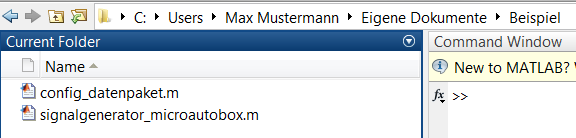
\includegraphics[scale = 0.65]{configfilespfad}
\caption[Verzeichniswechsel in MATLAB]{Verzeichniswechsel in MATLAB}
\label{configfilespfad}
\end{figure} 

Anschließend bewirkt die Eingabe von \textit{"`signalgenerator\_microautobox"} und \textit{"`config\_datenpaket"} im "Command Window", dass die Parameter der beiden Dateien in den Workspace von MATLAB geladen werden. Falls keine Tippfehler o.ä. aufgetreten sind, sollte nun im Workspace folgendes zu sehen sein: 

\begin{figure}[h]
\centering
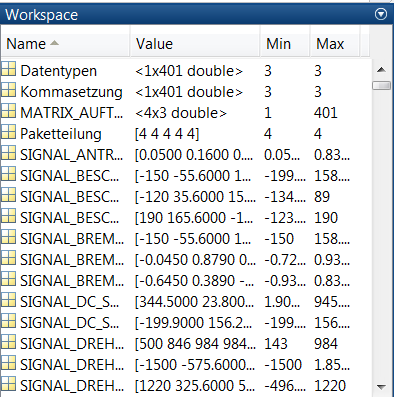
\includegraphics[scale = 0.65]{configfilesworkspace}
\caption[Parameter im Workspace]{Im Workspace enthaltene Parameter nach der Ausführung der beiden *.m-Files}
\label{configfilesworkspace}
\end{figure}  

\newpage

\textbf{Anmerkung:} Die Parameter "`Datentypen"\ , "`Kommasetzung"\ und "`Paketteilung" wurden nachträglich eingefügt, um den \textit{Encode32} - Block beim Enkodieren die korrekte Reihenfolge der Datentypen bei den zu übertragenden Paketinformationen mitzuteilen. Dies wird im Enkoder durch folgenden Vektor bei \textit{Datatype} vorgenommen: 

\begin{center}
$[ 4, \ 4, \ 4, \ Datentypen, \ Paketteilung, \ Kommasetzung ]$ 
\end{center}


 


%-------------------------------------------------------------------%

Abhängig von den weiteren Absichten des Benutzers werden im Folgenden nun für diese Ziele die jeweiligen Vorgehensweisen ausführlich erläutert. 

\subsection{Testen des Simulink-Modells durch den Signalgenerator}

Mittels des Simulink-Subsystems des Signalgenerators können dem Simulink-Modell beliebige, virtuell simulierte Werte zur Verfügung gestellt werden. Vor allem zur Validierung des Systems ist dies sehr sinnvoll, da es nicht nötig ist, die MicroAutoBox II in das Fahrzeug einzubauen bzw. Peripherie (Sensoren etc.) daran anzuschließen. Auch trägt dieser Simulink-Block stark zur Erweiterbarkeit und Wartbarkeit des Modells bei.  

\subsubsection{Modifizieren der Simulationswerte}

Um die vorhandenen Simulationswerte zu verändern gibt es zwei Möglichkeiten. 
Als erste Option steht eine direkte Änderung der Werte  der Parameter in den jeweiligen Source-Blöcken zur Verfügung. 
Die Anordnung der Blöcke ist im Entwurfsdokument genau erläutert. 
Die zweite Möglichkeit wäre die gewünschten Werte im \textit{*.m}-File \textit{signalgenerator\_microautobox.m} über die dazugehörigen Parameter zu verändern. 
Der Aufbau und Funktion dieses Files wurden hinreichend im Entwurfsdokument sowie im vorherigen Abschnitt beschrieben.


\subsubsection{Veränderungen am Modell} 

Bei Veränderungen des Simulink-Modells, um z.B. neue Sensorwerte aufzunehmen oder nicht mehr benötigte zu entfernen, bietet es sich an den Signalgenerator zu modifizieren und für Testzwecke zu verwenden. Dazu müssen die jeweiligen Werte aus dem Modell einschließlich des Signalgenerators entfernt oder hinzugefügt werden. Wichtig dabei ist, dass dies im kompletten Simulink-Model vorgenommen wird, da es sonst zu Fehlern kommt (s. hierzu Punkt 2.1.6). 


\subsubsection{Anschließen des Signalgenerator-Blockes an das Modell}

Falls sich im restlichen Modell keine Änderungen ergeben haben, stellt das erneute Anschließen des Signalgenerators kein großes Problem dar. 
Dieser muss einfach über eine Leitung mit dem Signalkollektor verbunden werden.  
Liegen jedoch Veränderungen vor, müssen diese, wie gerade erwähnt, komplett im Modell beachtet und bearbeitet werden. 
Dabei ist es wichtig, dass die Reihenfolge der Signale im Busarray analog zum Pflichtenheft erhalten bleibt (s. 2.1.4). 
Dabei spielt die Reihenfolge, in welcher die Signale über einen Bus-Creator gebündelt bzw. über einen Bus-Selector aufgespalten werden eine große Rolle. 
Die Signalreihenfolge kann innerhalb dieser Blöcke eingesehen und bearbeitet werden. 


\subsubsection{Verwenden des Signalgenerator-Blockes zu Testzwecken}

Ist das Modell nun komplett eingerichtet und mit dem Signalgenerator-Subsystem verbunden, ist es wichtig, dass das dazugehörige Datei signalgenerator\_microautobox.m ausgeführt wurde, damit die Parameterwerte der Signale MATLAB bekannt sind. Nach der Implementierung des Modells (s. 2.1.5) liegen die gewünschten Werte am Ausgang der MicroAutoBox II an und können an den Embedded-PC zur anschließenden Weiterverarbeitung der Fahrzeugdaten übertragen werden.


%-------------------------------------------------------------------%


\subsection{Anschluss des Simulink-Modells des Formula-Student-Fahrzeuges an das Simulink-Modell des Service Interfaces}

Um das Simulink-Modell des Formaula-Student-Fahrzeuges mit dem Simulink-Modell des Service Interfaces zu verbinden, sind folgende Schritte notwendig: \\

Zu Beginn muss als Vorbereitung das Subsystem \textit{Signalgenrator} vom Subsystem \textit{Signalcollector\_Embedded\_PC} getrennt und aus dem Modell entfernt werden. Des Weiteren empfiehlt es sich, die einzelnen Signale des Modells von Team StarCraft e.V. zu einem einzelnen Busarray zusammenzufassen und erst dann mit dem Busarray des Subsystems \textit{Signalcollector\_Embedded\_PC} zu verbinden.
Hierbei ist die Reihenfolge der im Pflichtenheft festgelegten Fahrzeugdaten einzuhalten (s. Abb. \ref{anschlussbus}) , um mögliche Fehler zu vermeiden. 

\begin{figure}[h]
\centering
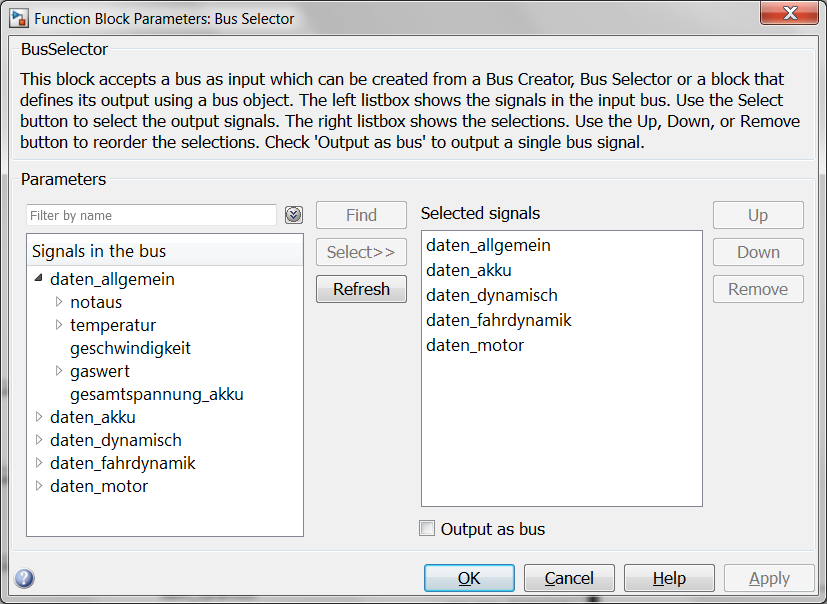
\includegraphics[scale = 0.45]{anschlussbus}
\caption[Einstellungen des Bus Creators]{Einstellungen des Bus Creators, um eine Verbindung der beiden Simulink-Modelle vorzunehmen}
\label{anschlussbus}
\end{figure} 

Wurde das Verbinden der beiden Modelle über ein Busarray korrekt durchgeführt, kann nunmehr mit Punkt 2.1.5 fortgefahren werden.


%-------------------------------------------------------------------%

\subsection{Implementierung des Modells auf der MicroAutoBox II}

Um das Simulink-Modell auf die MicroAutoBox II zu überspielen, müssen neben dem Modell auch die folgenden Dateien der Firma dSPACE in einem gemeinsamen Ordner liegen: 

\begin{itemize}

\item ds32encode.m
\item ds867c\_eth\_bit\_encoder\_sfcn.c
\item ds867c\_eth\_bit\_encoder\_sfcn.mexw32
\item ds867c\_eth\_encode32\_sfcn.c
\item ds867c\_eth\_encode32\_sfcn.mexw32

\end{itemize}

\textbf{Anmerkung:} Falls in einer späteren Erweiterung des Modells der UDP-Receive-Block benutzt werden sollte (dies wurde als alternatives Modell entworfen, aber aus Gründen der Robustheit wurde entgegen dem Feinentwurf auf eine bidirektionale Kommunikation verzichtet), so müssen darüber hinaus noch folgende Dateien dem Ordner hinzugefügt werden:

\begin{itemize}

% decoder *m. - file?

\item ds867c\_eth\_bit\_decoder\_sfcn.c
\item ds867c\_eth\_bit\_decoder\_sfcn.mexw32

\end{itemize}

Ist diese Voraussetzung erfüllt, so kann innerhalb von Simulink durch den Aufruf \\ \textit{Tools $\rightarrow$ Real-Time Workshop $\rightarrow$ Build Model} oder alternativ durch die Tastenkombination  \\ \textit{Strg + B} das Modell kompiliert und auf die MicroAutoBox II überspielt werden, was durchaus ein bis zwei Minuten in Anspruch nehmen kann. \\

\textbf{Anmerkung:} Sollten während des Kompilierens unerwartete Fehler wie z.B. folgende Meldung (s. Abb. ) auftreten, so liegt dies höchstwahrscheinlich an einer falsch eingestellten Message Size in den beiden UDP-Send-Blöcken \textit{ETHERNET\_UDP\_TX\_BL1} und \textit{ETHERNET\_UDP\_TX\_BL2} der Subsysteme \textit{UDP\_DATEN} und \textit{UDP\_PAKETINFORMATIONEN} (s. hierzu Punkt 2.1.1).

\begin{figure}[h]
\centering
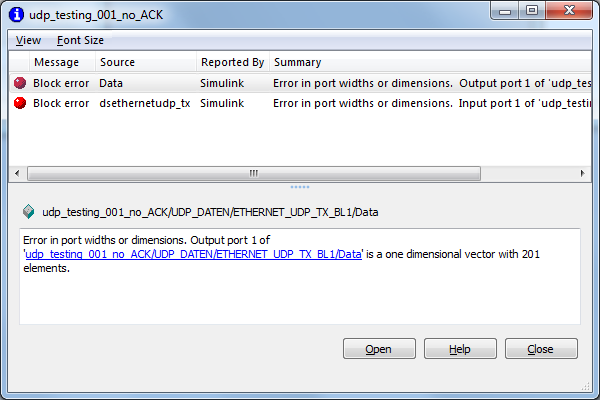
\includegraphics[scale = 0.48]{fehlermsgsize}
\caption[Fehlermeldung bei falsch konfigurierter Message Size]{Fehlermeldung bei falsch konfigurierter Message Size}
\label{fehlermsgsize}
\end{figure} 

\newpage

%-------------------------------------------------------------------%

\subsection{Appendix: Wichtige Hinweise zu dem Hinzufügen, Entfernen oder Modifizieren von Signalen}

Dieser Abschnitt soll dem späteren Nutzer wichtige Hinweise geben, an welchen Stellen Änderungen notwendig werden, sobald das Modell durch das Hinzufügen, Entfernen oder Modifizieren von Signalen verändert werden sollte. \\

Es empfiehlt sich, die folgende Checkliste abzuarbeiten, um mögliche Fehler beim Kompilieren einzugrenzen:

\begin{itemize}

\item Ist das Simulink-Modell korrekt an den Signalkollektor angeschlossen, d.h. die festgelegt Reihenfolge im Pflichtenheft eingehalten?

\item Wurden alle bereitgestellten Signale des Signalkollektors genutzt und falls nicht, wurden diese durch Terminatoren abgeschlossen oder durch vorher definierte Constant-Blöcke belegt?

\item Wurde für das Signal die richtige Verstärkung gewählt?

\item Liegen am Encoder-Block notwendigerweise die Daten im Datentyp \textit{double} vor?

\item Wurden die Signale im Encoder-Block korrekt in die entsprechenden Datentypen gewandelt (s. S.8 oben)?

\item Wurden in der *.m - File \textit{config\_datenpaket.m} die Vektoren korrekt an die Änderungen angepasst?

\item Wurde bei den UDP-Send-Blöcken die korrekte Message Size eingetragen?

\item Wurden bei den Einstellungen der Ethernet-Schnittstelle die korrekten Werte für die Remote IP etc. eingetragen?

\end{itemize}

\newpage

%-------------------------------------------------------------------%

\section{Embedded-PC}

%-------------------------------------------------------------------%

\section{vServer}

%Kurze Komponentenbeschreibung...

\subsection{Installation der Boost-Bibliotheken}

Boost stellt C++-Bibliotheken zur Verfügung, welche auf dem vServer zwingend benötigt werden.
Dazu muss auf beiden Systemen der folgende Befehl erfolgreich ausgeführt werden:
%1337 bitte Nachfolgendes als Konsolentext markieren:
    yum install boost boost-devel -y
    
Zur Installation über die Kommandozeile werden \textit{Administratorrechte} benötigt.

\subsection{Installation des MySQL-Connector/C++}

Der MySQL Connector/C++ ist zwingend erforderlich, damit das C++-Programm des virtuellen Servers auf die Datenbank zugreifen kann. Für die Installation benötigen Sie \textit{root}-Rechte, die folgenden Befehle werden in die Kommandozeile eingegeben.
Zuerst einmal muss sichergestellt werden dass alle im weiteren Verlauf verwendeten Programme vorhanden sind:\\
%1337 bitte Nachfolgendes als Konsolentext markieren:
  yum install bzr boost\_devel cmake mysql-devel –y \\

Anschließend kann der aktuelle Quellcode bezogen werden:\\
%1337 bitte Nachfolgendes als Konsolentext markieren:
  bzr branch lp:~mysql/mysql-connector-cpp/trunk ./mysql-connector-cpp \\

In das soeben Verzeichnis wechseln und die Makefile erstellen:\\
%1337 bitte Nachfolgendes als Konsolentext markieren:
  cd mysql-connector-cpp \\
  cmake . \\

Erstellung der Bibliotheken und Installation der Header-Dateien: \\
%1337 bitte Nachfolgendes als Konsolentext markieren:
  make clean \\
  make \\
  make install \\

Die Kompilierung des Programms kann einige Minuten in Anspruch nehmen. Für weitere Informationen, Testanleitungen und ggf. Fehlerbehandlung verweisen wir auf die MySQL-Dokumentation:

 http://dev.mysql.com/doc/refman/5.1/en/connector-cpp-installation-source-unix.html
 
 \subsection{Installation des auf dem vServer laufenden Programms}
 
 %Text hier: (Absprache mit Team C++ nötig)
 
 \subsection{Einstellungen über die Konfigurationsdatei}
 %Achtung, noch nicht final?
Die Konfigurationsdatei \textit{Konfiguration.conf} befindet sich im Installationsverzeichnis. Sie wird von dem Programm während der Laufzeit ausgewertet, damit können Programmparameter geändert werden, ohne das Programm neu kompilieren zu müssen.\\
In dieser Konfigurationsdatei werden die Zugangsdaten für die Datenbank, die Anzahl der in der Datenbank zu haltenden Datensätze sowie interne Parameter des Programms (IP-Adressen, Portnummern) festgesetzt.
Sollten Änderungen an diesen Parametern (beispielsweise bei der Anzahl) nötig sein, ist darauf zu achten, dass der Syntax der Datei erhalten bleibt und die Änderungen sowohl auf dem vServer als auch auf dem Embedded-PC eingepflegt werden.
Der jeweilige Parameter wird aus der auf die Beschreibung bzw. Nennung des Parameters folgenden Zeile ausgelesen. 
Diese darf nicht leer sein, auf Leerzeichen und zusätzliche Zeilenumbrüche sollte verzichtet werden.
Alle Zeilen, die mit einem Doppelkreuz (\#) beginnen, dürfen nicht verändert werden, da sonst das Programm die Parameter nicht mehr erkennt.

Beispielhafter Ausschnitt aus der Konfigurationsdatei:\\
%1337 bitte Nachfolgendes als Konsolentext markieren (und zwar alles...):

    \#Hostadresse der Datenbank\\
    localhost\\

    \#Name des Datenbankbenutzers\\
    telemetrie\\

    \#Passwort des Datenbankbenutzers\\
    fakePW\\

    \#Datenbankname\\
    telemetrie\\
%(... bis hier hin)

\textit{Wichige Anmerkungen:}\\
Stellen Sie sicher das alle Parameter korrekt gesetzt sind! Ansonsten kann ein störungsfreier Betrieb des Programms nicht gewährleistet werden!\\
Des weiteren ist darauf zu achten, das nur befugte Personen diese Datei einsehen können, da sie das Zugangspasswort zur Datenbank enthält!\\
Bei Fehler kann gegebenenfalls die Logdatei (log.txt im Installationsverzeichnis) nach Informationen durchsucht werden.

\subsection{Installation des Cronjobs}

Um die Datenbank in regelmäßigen Abständen auf ihre Größe zu prüfen und gegebenenfalls das Löschen von Einträgen zu veranlassen, wird ein Cronjob angelegt, durch den das eigenständige Programm \textit{StartResizeDB} in periodischen Zeitintervallen vom System aufgerufen wird.
Die Einrichtung des Cronjobs erfolgt manuell über die Kommandozeile des virtuellen Servers. Hierzu werden \textit{root}-Rechte benötigt.\\

Öffnen der Datei \textit{/ect/crontab} mit einem Editor (zum Bsp: \textit{nano}, \textit{vi}):\\

%1337 bitte Nachfolgendes als Konsolentext markieren:
  vi /etc/crontab    \\

Hier muss zuerst die Umgebungsvariable \textit{,,HOME"} gesetzt werden, damit das Programm nicht unter dem Wurzelverzeichnis ausgeführt wird. Der anzugebende Pfad ist abhängig vom Installationsverzeichnis und sollte auf den Überordner des Programms \textit{StartResizeDB} verweisen.\\
 
 %1337 bitte Nachfolgendes als Konsolentext markieren:
  HOME=/Pfad/zum/Installationsverzeichnis/

Nun wird an das Ende der Datei folgende Zeile hinzugefügt, wobei der Pfad zu ersetzen ist:\\

%1337 bitte Nachfolgendes als Konsolentext markieren:
  0 * * * * root /Pfad/zur/StartResizeDB 2\textgreater\&1 \\

Der anzugebende Pfad ist abhängig vom Installationsverzeichnis und sollte auf die Datei \textit{StartResizeDB} verweisen.
Damit wird das angegebene Programm zu jeder vollen Stunde ausgeführt, \textit{,,root"} ist hier der ausführende Benutzer. Der angegebene Benutzer sollte Rechte zum Lesen und Schreiben auf alle Projektdateien besitzen.\\
\textit{,,2\textgreater\&1"} bedeutet, dass die Cron-Standardausgabe benutzt wird.
Es ist auf genaue Einhaltung des Syntax zu achten.\\
Beim anschließenden Speichern und Schreiben der Datei wird der Cronjob automatisch installiert.

%-------------------------------------------------------------------%

\section{Datenbanken}

\subsection{Fahrzeugdatenbank}

\subsection{Benutzerdatenbank}

%-------------------------------------------------------------------%



\newpage

% Text von Thomas eingepflegt, gez. Sebastian

\section{Webseite}

Zur uneingeschränkten Nutzung der Software müssen einige Voraussetzungen erfüllt sein: 

\begin{itemize}

\item Webserver 

\begin{itemize}

\item PHP Version 5.3 oder höher
\item mindestens eine (idealerweise zwei) MySQL-Datenbank (MySQL Version 5.3 oder höher)
\item SMTP-Server mit Authentifizierung
\item X MB freien Speicherplatz für Webseite

\end{itemize}

\end{itemize}

Im Folgenden werden alle nötigen Installationsschritte für die gesamte Software sowie die entsprechenden Konfigurationseinstellungen erläutert, welche zu Beginn getroffen werden müssen. \\

\textit{Webseite - Konfiguration} \\

Alle ausgelieferten Verzeichnisse und Dateien müssen in das Stammverzeichnis (s. Beschreibung Ihres Hostingangebotes) hochgeladen werden. Bevor Sie dies jedoch tun, müssen sie die Datei \textit{includes/config.php} anpassen. \\ 

\begin{figure}[h]
\centering
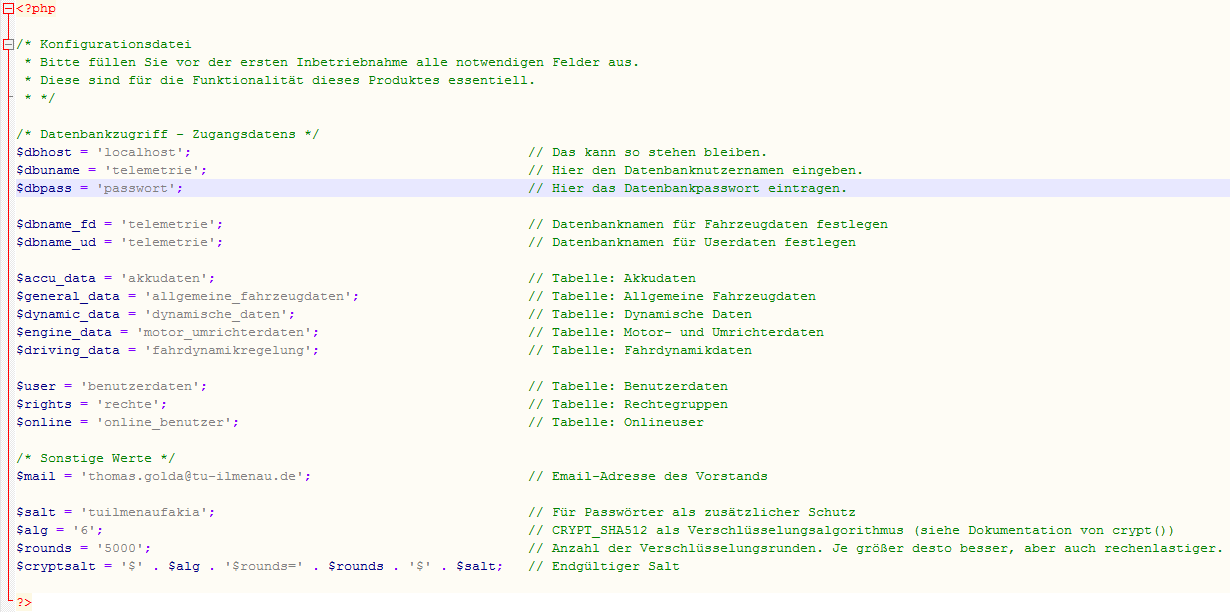
\includegraphics[scale = 0.50]{website_config}
\caption[Auschnitt aus der config.php - Datei]{Auschnitt aus der config.php - Datei}
\label{websiteconfig}
\end{figure} 

\newpage

Für Sie sind lediglich sechs Zeilen wichtig: 

\begin{itemize}[leftmargin=*]

\item \textit{\$dbhost}: Diese Einstellung ist auf "`localhost"\ gestellt. In den meisten Fällen ist dies die Standardeinstellung. Sollten Sie von Ihrem Provider explizit andere Angaben erhalten haben, dann ändern Sie dieses Feld. Sollten Sie keine Informationen erhalten haben, wird mit hoher Wahrscheinlichkeit "`localhost"\ die richtige Wahl sein. Sollte es zu Problemen kommen, setzen Sie sich bitte mit Ihrem Provider in Verbindung.


\item \textit{\$dbuname}: Hier fügen Sie in einfachen Anführungszeichen den Ihnen vom Provider mitgeteilte Zugangsnamen für den Datenbankserver ein.


\item \textit{\$dbpass}: Hier fügen Sie entsprechend das an Sie vergebene Passwort für die Datenbank ein.

\item \textit{\$dbname\_fd}: Sollten Sie vom Provider bereits eine Datenbank erhalten haben, so fügen Sie hier den Namen der Datenbank ein. Wenn Sie vollen Zugriff auf den Datenbankserver haben und selber Datenbanken anlegen können, so steht es Ihnen frei, wie Sie die Datenbank der Fahrzeugdaten bezeichnen möchten.


\item \textit{\$dbname\_ud}: Sollten Sie vom Provider bereits eine Datenbank erhalten haben, so fügen Sie hier den Namen der Datenbank ein. Wenn Sie vollen Zugriff auf den Datenbankserver haben und selber Datenbanken anlegen können, so steht Ihnen die Wahl frei, wie Sie die Datenbank der Nutzerdaten bezeichnen möchten.

\textbf{Anmerkung:} Beide Datenbanknamen können identisch sein, z.B. wenn Sie von Ihrem Provider nur eine Datenbank erhalten haben sollten. 

\item \textit{\$mail}: Hier tragen Sie bitte die E-Mail-Adresse des Vorstandes ein. Alle eingehenden Registrierungsanfragen werden an diese E-Mail-Adresse weitergeleitet. Diese kann auch nach der Installtion noch angepasst werden. Alle anderen Werte müssen ab dem Beenden der Installation unverändert bleiben um die volle Funktionsfähigkeit gewährleisten zu können.

\end{itemize}

\newpage


\textit{Webseite - Installation} \\

Nachdem die Konfiguration erfolgreich durchgeführt wurde, öffnen Sie die Webseite in einem Browser und geben manuell den Pfad \textit{,,install.php"} zusätzlich zur Adresse der Webseite in die Suchleiste ein.\\
Pfadbeispiel: \textit{team-starcraft.de/swp\_formula\_student/install.php} - dabei ist \textit{swp\_formula\_student} das Hauptverzeichnis der Webseite. \\
 Danach füllen Sie das entsprechende Formular aus und schicken dieses ab. 
 Anschließend werden alle nötigen Datenbanken und Tabellen erzeugt, sowie die Nutzergruppen und der Vorstandsaccount eingerichtet.

\begin{figure}[h]
\centering
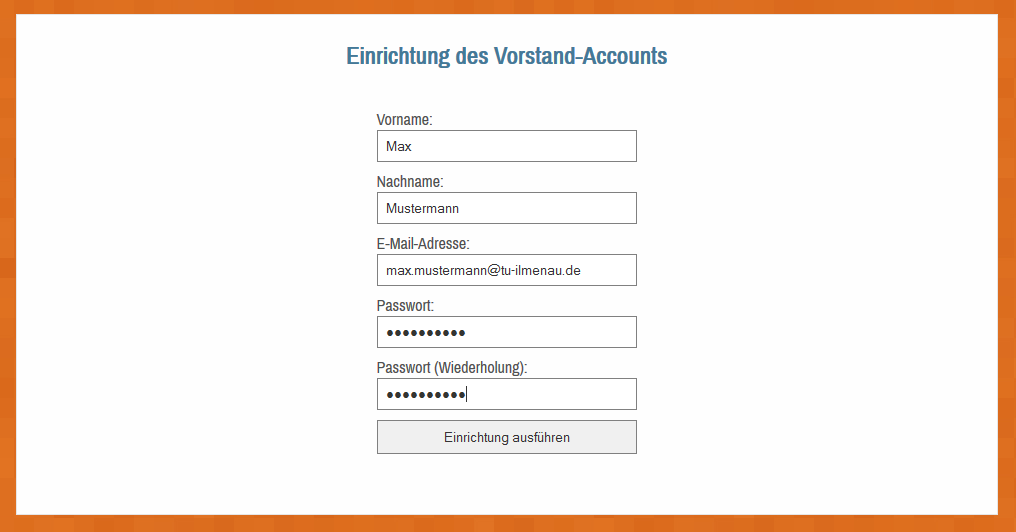
\includegraphics[scale = 0.50]{install}
\caption[Einrichtung des Vorstand - Accounts]{Einrichtung des Vorstand - Accounts}
\label{installvorstand}
\end{figure} 


Sollten Sie von Ihrem Provider bereits Datenbanken erhalten haben, tritt nach der Installation ein Fehler mit der Meldung auf, dass die zu erstellende Datenbank bereits existiert. Dies ist normal und kein Grund zur Sorge. \\ \\

Die Installation ist nun vollständig. Bitte löschen Sie die \textit{install.php} unverzüglich vom Server um Missbrauch zu vermeiden. Sie können Sich nun mit den angegeben Zugangsdaten einloggen.




%----------------- Bedienung des Service-Interfaces ----------------%

\chapter{Bedienung des Service-Interfaces}

\section{Startseite / Verwaltung}

Über die Startseite loggen Sie sich mit den Zugangsdaten mit denen Sie sich registriert haben ein. 
Ob Ihr Account bereits freigeschaltet wurde, erfahren Sie vom Vorstand. 
Nach dem Einloggen werden hier allgemeine Informationen dargestellt, wie z.B. eine Liste der sich zur Zeit online befindlichen Nutzer und eine Exportfunktion zum Extrahieren der Fahrzeugdaten aus der Datenbank. 
Als Vorstand erhalten Sie zudem noch eine Liste sämtlicher registrierter Nutzer und eine Möglichkeit Nutzer freizuschalten bzw. zu löschen und Rechtegruppen zu vergeben oder zu ändern. \\

\textbf{Anmerkung:} Bitte verwenden Sie für die Registrierung im Service Interface entweder Ihre E-Mail-Adresse vom Team Starcraft, eine TU Ilmenau E-Mail-Adresse oder eine 1und1-Adresse um möglichen Problemen aus dem Weg zu gehen.

\section{Nutzerverwaltung (Vorstand)}

Wenn Sie einen Nutzer bearbeiten wollen, muss stets eine der beiden Radioboxen aktiviert sein und im Textfeld seine ID-Nummer eingetragen werden. Möchten Sie einen Nutzer löschen, so wählen sie "`Löschen"\ , möchten Sie ihn jedoch aktivieren oder bearbeiten, so wählen Sie "`Aktivieren"\ aus. Mittels des Dropdown-Menüs können Sie dem Benutzer eine Rechtegruppe zuweisen. \\ \\
\textbf{Achtung:} Sie können sich nicht selbst löschen, dies muss ein anderer Nutzer mit Vorstandsrechten für Sie erledigen!

\section{CSV-Export}

Durch Auswahl einzelner Checkboxen können Sie sich die Daten des Fahrzeugs als \\ CSV-Datei herunterladen. Aus technischen Gründen kann es beim Auswählen mehrerer Boxen dazu kommen, dass Datensätze fehlen. Dies können Sie vermeiden, indem sie die Tabellen einzeln exportieren.

\section{Passwort ändern}

Diese Seite ermöglicht es Ihnen Ihr Passwort - beispielsweise nach einem Reset - zu ändern. Sie erreichen diese über die unter dem Hauptmenü befindlichen Link "`Passwort ändern".

\section{Passwort vergessen}

Auf der Startseite befindet sich ein Link "`Passwort vergessen". Klicken Sie auf ihn und geben Sie ihre Emailadresse ein. Bei erfolgreicher Änderung des Passworts erhalten Sie das neue Passwort per Mail zugeschickt. Andernfalls erscheint eine Fehlermeldung.

\section{Menüleiste}

Über die Menüleiste können Sie die einzelnen Unterseiten aufrufen. Jede Unterseite stellt eine andere Gruppe von Fahrzeuginformationen dar (s. Pflichtenheft). \\ \\

Es ist zu Empfehlen sich nach jedem Besuch der Seite wieder auszuloggen.


%----------------------  Abbildungsverzeichnis  --------------------%

\listoffigures

\addcontentsline{toc}{chapter}{Abbildungsverzeichnis}


\end{document}